\section{Aufbau der Wetterstation und Sensoren}


%% ###################################################################################################
%%   Unterkapitel                                                                                                                                                                              #
%% ###################################################################################################
\subsection{Übersicht der Hardware}
Die Wetterstation Arbon verfügt über fünf Sensoren bzw. Sensor-Einheiten: Webcam, Kombi-Wetter-Transmitter, Wassertemperatur-Sensoren, Pegelsensor und Sonnenstrahlungssensor. Auf der Plattform im See draussen befindet sich lediglich ein Schaltschrank mit Datenwandlern und keine Auswerteeinheit. Sämtliche Daten werden per TCP/IP an den Server geschickt. Abbildung \ref{img:schaltschrank} zeigt den schematischen Aufbau der Komponenten im Schaltschrank und die angeschlossenen Sensoren. Die Stromversorgung ist der Übersicht halber nicht dargestellt.

\Diskussionspunkt{- Strahlungssensor hinzufügen}\newline

\begin{figure}[ht]
	\centering
	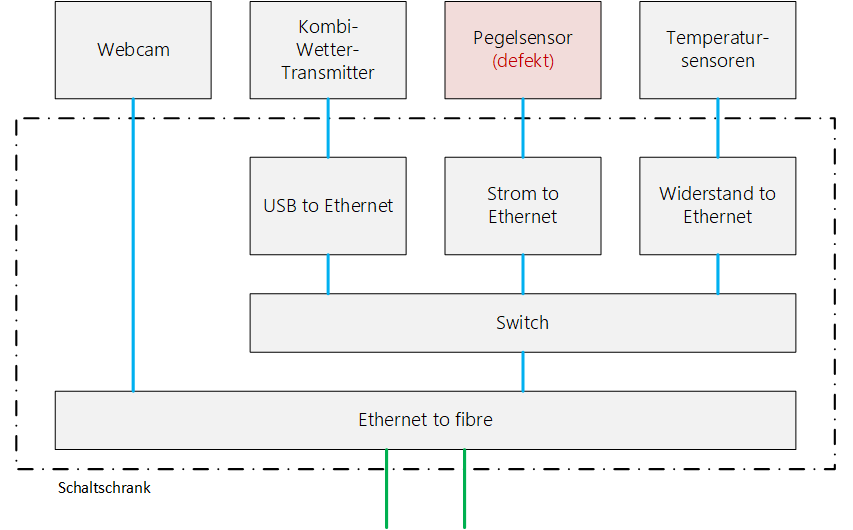
\includegraphics[width=0.9\linewidth]{img/schaltschrank.png}
	\caption{Hardware-Aufbau der Wetterstation Arbon}
	\label{img:schaltschrank}
\end{figure}

%% ###################################################################################################
%%   Unterkapitel                                                                                                                                                                              #
%% ###################################################################################################
\subsection{Sonnenstrahlungssensor}
Die Sonnenscheindauer dient der näherungsweisen Abschätzung der Einstrahlung an einem bestimmten Ort und gibt gleichzeitig Hinweise auf Zeit und Stärke der Bewölkung. Die Angabe der Sonnenstunden diente ursprünglich der Charakterisierung von Kurorten. Dabei wurde die psychologische Wirkung von Sonnenlicht auf das menschliche Wohlbefinden hervorgehoben. Die Sonnenstunden werden heute immer noch verwendet um touristische Ziele zu fördern. 

\noindent
Zur Messung der Sonnenstunden gibt es gemäss  \flqq Guide to Meteorological Instruments and Methods of Observation\frqq ~\cite{WMO2014Gtmi}  fünf Messprinzipien, wobei die pyranometrische Methode, die einfachste und kostengünstigste Methode darstellt. Gemäss WMO~\cite{WMO2014Gtmi} Kapitel 8.1.4 kann die Sonnenscheindauer durch die Messung der globalen Sonneneinstrahlung $G$ abgeschätzt werden. Die Globalstrahlung wird dabei von einem Pyranometer gemessen.

\subsubsection{Funktionsprinzip eines Pyranometers}
Das Pyranometer basiert auf dem Messprinzip eines Thermoelements, wie in Abbildung \ref{img:pyranometer}  dargestellt. Die eintreffende Strahlung trifft auf einen Absorber, welcher erwärmt wird. Die Wärme „fliesst“ dann über das Gehäuse an die Umgebung ab. Die Strahlungsleistung ist proportional zum Wärmestrom bzw. zur Temperaturdifferenz vom Absorber zum Gehäuse. Die Temperaturdifferenz wird mit Thermoelementen gemessen. Um die Signalspannung zu erhöhen werden mehrere Thermoelemente in Reihe geschalten, welches Thermosäule genannt wird. Durch das thermische Messprinzip ist ein Pyranometer träge. Die Response time liegt bei wenigen Sekunden. Das schwarz-poröse Absorbermaterial muss eine hohe Langzeitstabilität insbesondre gegenüber kurzwelliger Strahlung aufweisen. 

\begin{figure}[ht]
	\centering
	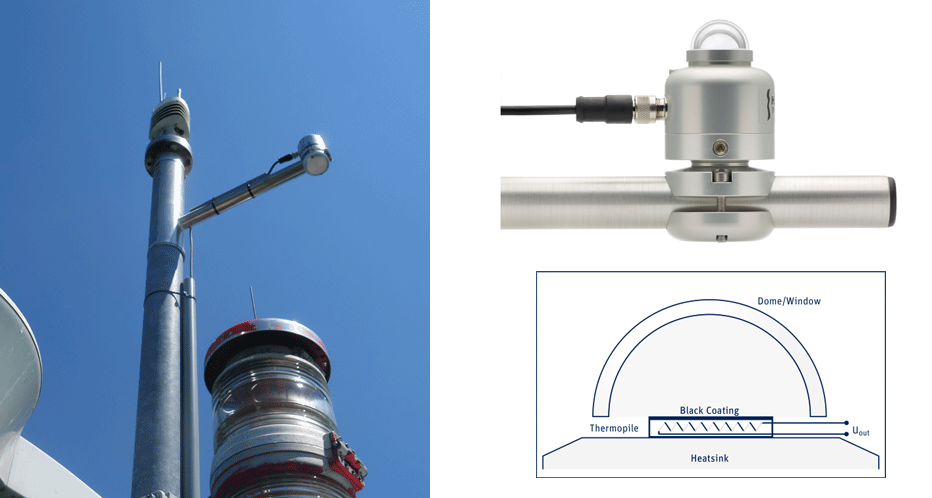
\includegraphics[width=0.9\linewidth]{img/pyranometer.png}
	\caption{Pyranometer}
	\label{img:pyranometer}
\end{figure}
%Quelle: http://www.kippzonen.com/News/572/The-Working-Principle-of-a-Thermopile-Pyranometer#.WzuK8C35ybg

\subsubsection{Berechnung der Sonnenscheindauer}
Die (relative) Sonnenscheindauer beschreibt den Anteil der tatsächlichen an der effektiv möglichen Sonnenscheindauer in Prozent. Durch sie kann man Sonnenscheinverhältnisse verschiedener Gebiete vergleichen. Gemäss ANNEX 8.B. der Richtlinie ~\cite{WMO2014Gtmi} kann die Sonnenscheindauer aus den minütlichen Messwerten der Globalstrahlung berechnet werden. Dazu muss zuerst der Schwellwert, wie in \ref{eq:Sonnenstunden} dargestellt, berechnet werden. Der Zähler für die Sonnenstunden wird um eine Minute erhöht, wenn der Messwert grösser ist als der Schwellwert und der Sonnenwinkel mindestens 3 Grad beträgt.\newline

\begin{equation}
\label{eq:Sonnenstunden}
G_{thr} = A + B * cos(\frac{360*d}{24*365}) * 1080 * sin(h)^{1.25}
\end{equation}

wobei:
\begin{conditions}
G_{thr}       &  Schwellwert der Globalstrahlung \\
d        &  Laufende Stunde seit Anfang Jahr \\
h        &  Elevationswinkel der Sonne in Grad \\
A        &  empirisch bestimmter Koeffizient (0.65) \\
B        &  empirisch bestimmter Koeffizient (0.15) \\
\end{conditions} 

%Die physikalische Größe der Sonnenscheindauer (SD) ist Zeit. Die verwendeten Einheiten sind Sekunden oder Stunden.
%Der Messzeitraum (Tag, Dekade, Monat, Jahr usw.) ist ein wichtiger Zusatz zur Einheit.

\noindent
Wenn der Winkel $h$ grösser oder gleich 3 Grad ist, und der gemittelte Minutenwert der Solarstrahlung höher ist als der Schwellwert, wird der Zähler für die Sonnenstunde um eine Minute erhöht.

%Guten Tag Frau Bilgery,
%scheint grössere Abweichungen zu geben. Habe es mit zwei anderen Datensätzen versucht mit dem ähnlichen Ergebnis.
%
%Im beiliegenden File habe ich die Strahlung bei einer Sonnenhöhe <3 Grad auf Null gesetzt, d.h. Morgen und Abendstunden werden nicht berücksichtigt. Fehler mit Division von sin(h) gibt es dann auch nicht.
%Für Buchs ist dies zulässig da die umliegenden Berge über einem Höhenwinkel von 3 Grad liegen. Dies wird aber in der Literatur auch für südliche Regionen ohne Berge durchgeführt. D.h. dies ist eine Massnahme. Weitere Massnahme ist die Reduktion der Faktoren A und B bis die Werte übereinstimmen.
%
%Faktor B-Reduktion kann beurteilt werden, wenn ein Sommertag und Wintertag betrachtet wird, da dieser die Saisonalität bestimmt.


\subsubsection{Verwendung für PV-Anlagen}
\Diskussionspunkt{- Wann reicht Globalstrahlung, wann wird Direktstrahlung benötigt?}\newline
\Diskussionspunkt{- Was kann in PV-Berechnungstools eingegeben werden?}\newline


%% ###################################################################################################
%%   Unterkapitel                                                                                                                                                                              #
%% ###################################################################################################
\subsection{Pegelsensor und Wellenhöhenmessung}
\Diskussionspunkt{- Pegelmessung, Pegelberechnung, Wellenhöhenberechnung}\newline
\Diskussionspunkt{- Gegenüberstellung Messprinzipien, Vor- und Nachteile}\newline
\Diskussionspunkt{- Unterschied Wellenhöhe und Seegang}\newline


\subsubsection{Auswahl eines Pegelsensors}
Für die Messung des Bodensee-Pegels wurden verschiedene Messprinzipien verglichen, mit dem Hintergedanken die Pegelmesswerte ebenfalls zur Messung der Wellenhöhe verwenden zu können.

\begin{table}[htb!]
\setlength\extrarowheight{3pt} % for a more "open" look
\begin{tabularx}{\textwidth}{|>{\RaggedRight\hspace{0pt}}p{1.5cm}||X|X|}
\hline
 & \bfseries\large Vorteile & \bfseries\large Nachteile\\

\hline
\textbf{Hydrostatisch}
&
\begin{itemize}[nosep,leftmargin=*]
\item einfache Auswertung
\item mechanische Dämpfung
\item sehr kleiner Energieverbrauch
\end{itemize}
&
\begin{itemize}[nosep,leftmargin=*]
\item anfällig auf Verschmutzung
\item keine Wellenmessung möglich
\end{itemize}\\

\hline
\textbf{Ultraschall}
&
\begin{itemize}[nosep,leftmargin=*]
\item berührungslos
\item geringer Energiebedarf
\end{itemize}
&
\begin{itemize}[nosep,leftmargin=*]
\item anfällig auf Wind
\end{itemize}\\

\hline
\textbf{Radar}
&
\begin{itemize}[nosep,leftmargin=*]
\item windunabhängig
\item berührungslos
\end{itemize}
&
\begin{itemize}[nosep,leftmargin=*]
\item zu geringe Auflösung für Wellenhöhe
\item hoher Energiebedarf
\end{itemize}\\

\hline
\textbf{TOF}
&
\begin{itemize}[nosep,leftmargin=*]
\item Wellenhöhe messbar
\item berührungslos
\end{itemize}
&
\begin{itemize}[nosep,leftmargin=*]
\item komplexe Auswertung
\end{itemize}\\

\hline
\textbf{Boje}
&
\begin{itemize}[nosep,leftmargin=*]
\item Wellenhöhe messbar
\end{itemize}
&
\begin{itemize}[nosep,leftmargin=*]
\item wartungsintensiv
\item Batteriebetrieb
\end{itemize}\\


\hline
\end{tabularx}
\end{table}

Der Pegelsensor liefert 4...20mA bei einer Messhöhe von 6 Meter. Der Pegelsensor ist ??? Meter über dem Pegelnullstand (Definition!!!) angebracht.
Für die Berechnung des Bodensee-Pegels aus dem Messwert ergibt sich analog der Geradengleichung $ y = m * x + q  $ wie in der Formel \ref{eq:Pegelformel} dargestellt.

\begin{equation}
\label{eq:Pegelformel}
Pegel [m] = 6m/16mA * Messwert [mA] + ???m
\end{equation}

\subsubsection{Definition des Bodenseepegels}
\Diskussionspunkt{- Wie ist der Bodenseepegel definiert? Quelle?}\newline

\subsubsection{Definition der signifikaten Wellenhöhe}
\Diskussionspunkt{- siehe List of Sea state Parameter 1986 }\newline


%% ###################################################################################################
%%   Unterkapitel                                                                                                                                                                              #
%% ###################################################################################################
\subsection{Wassertemperatur-Sensoren}
\Diskussionspunkt{- Funktionsweise, Aufbau der Wassertemperaturmessung}\newline
\Diskussionspunkt{- Berechnung, Verlauf der Wassertemperatur in Abhängigkeit der Tiefe}\newline
\Diskussionspunkt{- Wo ist Wassertemperatur definiert? Warum 1m unter der Oberfläche? Warum brauchen wir 0.5m unter Wasseroberfläche}\newline
\Diskussionspunkt{- Foto Verwendung Seebad Arbon}\newline


\subsubsection*{Auswahl des richtigen Temperatursensors anhand des Pegels}
\Diskussionspunkt{- Welcher Sensor muss auf Grund des Pegels ausgewählt werden -> Skizze}\newline
\Diskussionspunkt{- Codesniplet}\newline
Um die richtige Temperaturen bestimmen zu können ist der Pegel notwendig, hierfür wird im Cronjob zuerst den Pegel ausgelesen und anschliesend mittels der if Funktion, dies musste mit einem if gemacht werden, da Python keine cases kennt, den richtigen Sensor ausgewählt.

\begin{lstlisting}

\end{lstlisting}

\begin{figure}[h]
	\centering
	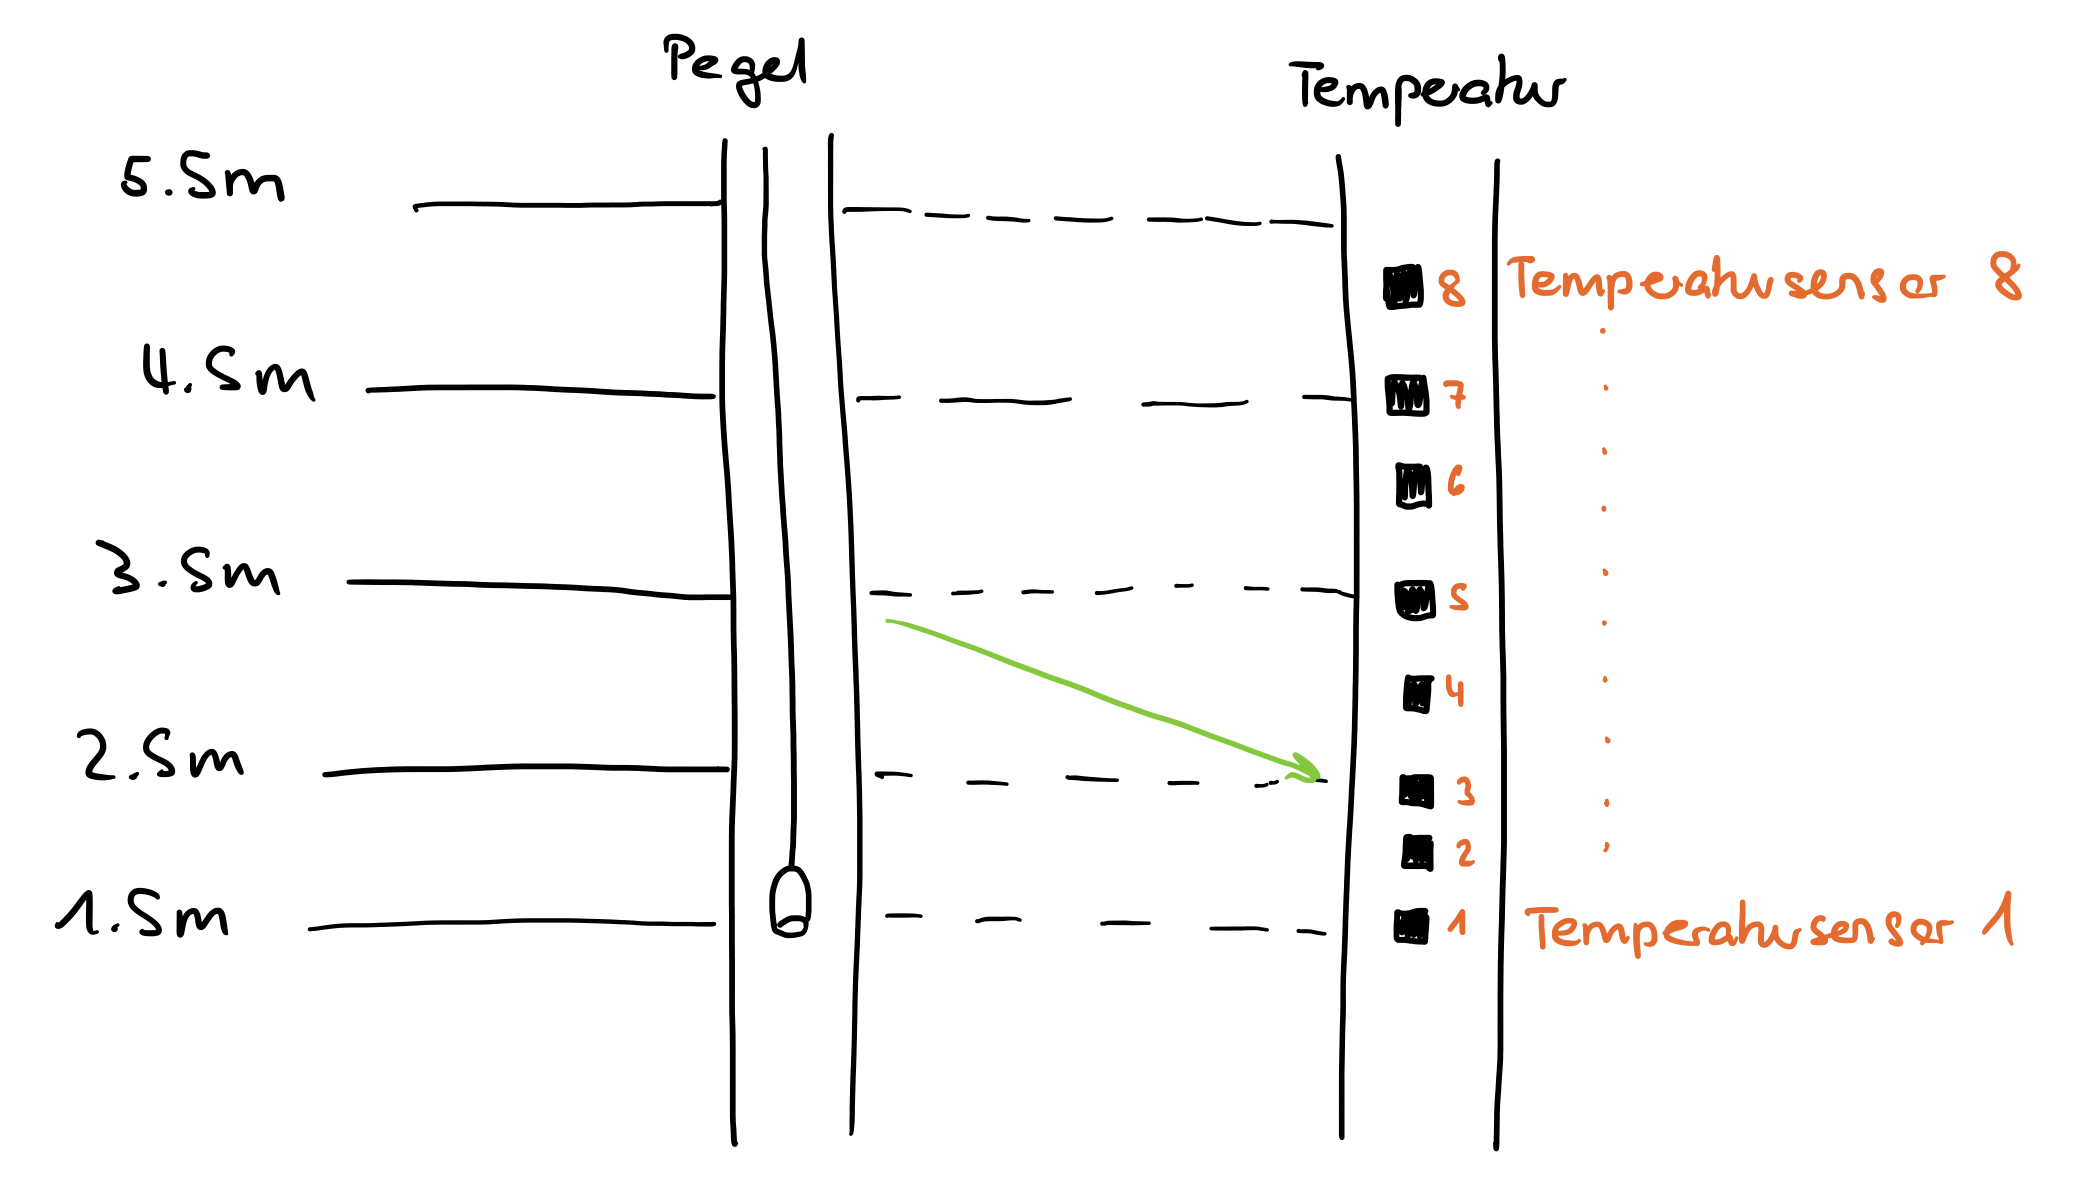
\includegraphics[width=0.9\linewidth]{img/wassertempsensoren.png}
	\caption{Zusammenhang zwischen Pegel und PT100-Temperaturwiderständen}
	\label{img:wassertempsensoren}
\end{figure}


\subsubsection*{Kompensation des defekten PT100-Widerstands}
\Diskussionspunkt{- Offset des defekten Sensors}\newline
\Diskussionspunkt{- Grafik der aufgezeichneten Daten -> kein klarer Offset vorhanden!}\newline
\Diskussionspunkt{- Wie wurde Problem gelöst -> Code}\newline








